
\begin{question}
A thief is filling her backpack with two types of valuable substances.
She can carry up to 40 kg, and her backpack can fit up to 10 liters.

Each bag of \(X\) has a weight of 9 kg, volume of 0.8 L, and value of 80
thousand USD.

Each bag of \(Y\) has a weight of 0.08 kg, volume of 0.03 L, and value
of 0.8 thousand USD.

There is no requirement to take full bags, so the thief can opt for a
fraction of a bag.

How many bags of each should the thief take to maximize her profit?
\end{question}

\begin{solution}
The thief should take 1.94 bags of \(X\) and 281.55 bags of \(Y\). We
can use linear programming to see this.

We write a weight inequality. \[9x+0.08y \le 40\] We write a volume
inequality. \[0.8x+0.03y \le 10\] We graph the two inequalities, shading
the feasible region.

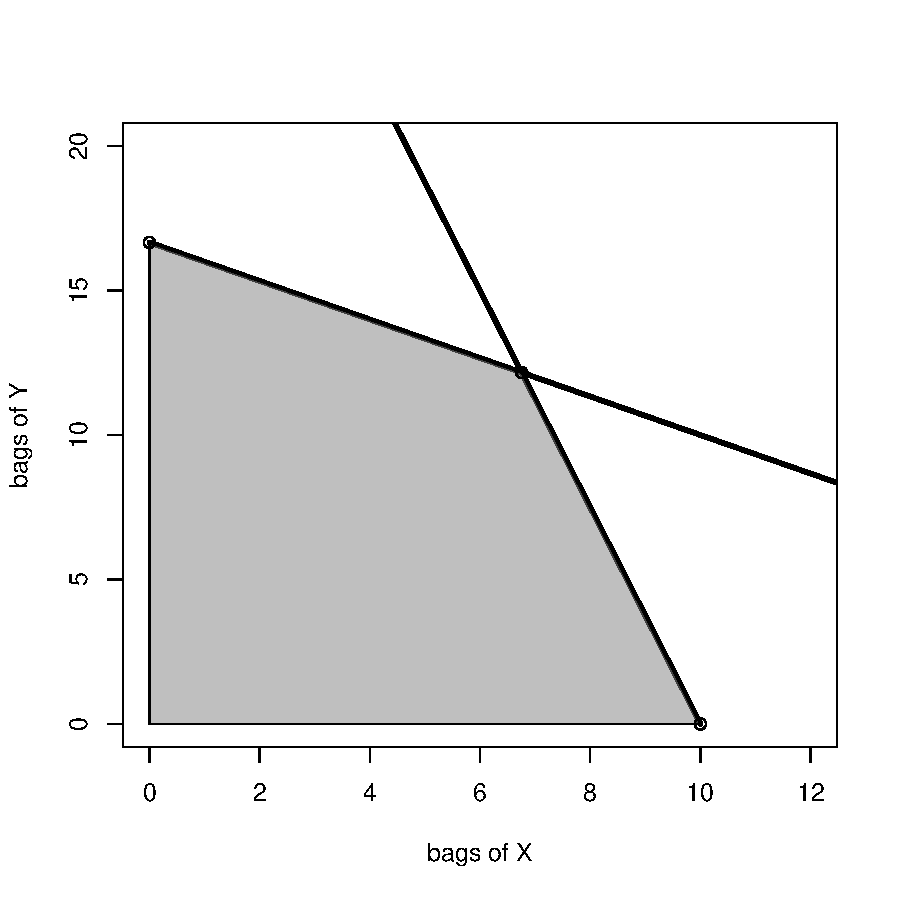
\includegraphics{unnamed-chunk-1-1.pdf}\\

There are three vertices of interest. \[(0,333.33) \] \[(1.94,281.55) \]
\[(4.44,0)\]

We write a profit function (the objective function).
\[P(x,y) = 80x+0.8y \]

We determine the profits. \[P(0,333.33)=266.67 \]
\[P(1.94,281.55)=380.58 \] \[P(4.44,0)=355.56 \] Thus, the thief should
take 1.94 bags of \(X\) and 281.55 bags of \(Y\).
\end{solution}

